\subsection{Model results}
\label{sec:model_results}

\paragraph{Training} The strategy has been optimized using a random search in
the hyperparameter space as commented in section \ref{sec:methods_pipeline_training}.
Primary model results are shown in table \ref{table:primary_model_hyperparameters},
and secondary model results are shown in table \ref{table:secondary_model_hyperparameters}.

\begin{table}[H]
  \centering
  \begin{tabular}{|c | c |} 
    \hline
    \multicolumn{2}{|c|}{Primary model} \\
    \hline
    Parameter & Value \\
    \hline
    Moving average fast window length & 5 \\
    \hline
    Moving average slow window length & 30 \\
    \hline
    Profit taking band                & 0.06 \\
    \hline
    Stop loss taking band             & 0.02 \\
    \hline
    Triple barrier window length      & 3 \\
    \hline
    Minimum return                    & 0.005 \\
    \hline
    Volatility window length          & 50 \\
    \hline 
  \end{tabular}
  \caption{Primary model hyperparameters.}
  \label{table:primary_model_hyperparameters}
\end{table}

\begin{table}[H]
  \centering
  \begin{tabular}{|c | c |} 
    \hline
    \multicolumn{2}{|c|}{Secondary model} \\
    \hline
    Parameter & Value \\
    \hline
    Number of estimators                & 720 \\
    \hline
    Maximum features ratio when bagging & 0.2936 \\
    \hline
    Average uniqueness                  & 0.9502 \\
    \hline
    Cross validation splits             & 6 \\
    \hline
    Embargo                             & 1\% \\
    \hline
  \end{tabular}
  \caption{Secondary model hyperparameters.}
  \label{table:secondary_model_hyperparameters}
\end{table}

\paragraph{Labels} The output of the primary model is summarized in table
\ref{table:labels_metalabel} where we also show the labels and metalabels count.
Also, in \ref{table:label_vs_metalabel} a contingency table between 
labels and metalabels is shown. We can see that even though labels are balanced,
there is a bias towards negative metalabels (i.e. do not take the bet) based on
the triple barrier parameters.

\begin{table}[H]
  \centering
  \begin{tabular}{| c | c |} 
    \hline
    \multicolumn{2}{|c|}{Labels}      \\
    \hline
    Value & Count                     \\
    \hline
    1 (buy signal) & 80               \\
    \hline
    -1 (sell signal) & 79             \\
    \hline
    \multicolumn{2}{|c|}{Metalabels}  \\
    \hline
    Value & Count                     \\
    \hline
    0 (unreliable label)     & 103    \\
    \hline
    1 (reliable label)       & 56     \\
    \hline
  \end{tabular}
  \caption{Primary model labels and metalabels.}
  \label{table:labels_metalabel}
\end{table}

\begin{table}[H]
  \centering
  \begin{tabular}{|c|c|c|}
    \hline
    Label     & \multirow{2}{*}{0} & \multirow{2}{*}{1} \\ \cline{1-1}
    Metalabel &                    &                    \\ \hline
    1         & 51                 & 29                 \\ \hline
    -1        & 52                 & 27                 \\ \hline
  \end{tabular}
  \caption{Contingency table between labels and metalabels.}
  \label{table:label_vs_metalabel}
\end{table}

\paragraph{Feature importance} Table \ref{table:feature_importance_results}
shows the mean loss in performance per feature after applying the method explained in
\ref{sec:methods_pipeline_feature_importance}. Note that only those features
with mean loss in performance above the mean loss are shown. See figure
\ref{fig:feat_importance} for an in detail mean loss of performance and standard
deviation per feature permutation.

It is interesting to point the groups of features that remained in the final model:

\begin{itemize}
  \item Price and volume features with fractional differentiation.
  \item SADF derived indices with different regression models (constant, linear and
        quadratic) and with one, two and three lag periods for the autocorrelation.
  \item Volatility and logarithmic returns.
  \item Market capitalization.
  \item Fees, transfer volume and days till halving. These are features related
        to the bitcoin ecosystem. 
\end{itemize}

However, none of the social features seemed to produce a high impact in the final
model.

\begin{table}[H]
  \centering
  \begin{tabular}{| c | c | c |} 
    \hline
    \multicolumn{3}{|c|}{Feature importance} \\
    \hline
    Feature                     & Mean perf. loss & Std. dev. of perf. loss\\ \hline
    CloseFFD                    & 0.039714        & 0.026393 \\ \hline
    HighFFD                     & 0.018739        & 0.019605 \\ \hline
    LowFFD                      & 0.002177        & 0.001215 \\ \hline
    OpenFFD                     & 0.006869        & 0.003897 \\ \hline
    Volume\_(BTC)-log            & 0.032430        & 0.015899 \\ \hline
    Volume\_(Currency)-log       & 0.020350        & 0.008696 \\ \hline
    bsadf\_ct\_1                  & 0.002128        & 0.002060 \\ \hline
    bsadf\_ctt\_1                 & 0.003910        & 0.003278 \\ \hline
    bsadf\_ctt\_2                 & 0.004907        & 0.004139 \\ \hline
    bsadf\_ctt\_3                 & 0.003264        & 0.004178 \\ \hline
    bsadf\_nt\_2                  & 0.003447        & 0.004077 \\ \hline
    daysTillHalving             & 0.003387        & 0.003194 \\ \hline
    fees-mean-log               & 0.004142        & 0.002743 \\ \hline
    log\_ret                     & 0.013930        & 0.006140 \\ \hline
    market-cap-log              & 0.002412        & 0.001501 \\ \hline
    transfer-volume-median-log  & 0.006073        & 0.006431 \\ \hline
    trgt                        & 0.003003        & 0.007776 \\ \hline
    vol\_15                      & 0.008678        & 0.003120 \\ \hline
    vol\_5                       & 0.020516        & 0.015831 \\ \hline
  \end{tabular}
  \caption{Feature performance loss of the secondary model. Only selected features are displayed.}
  \label{table:feature_importance_results}
\end{table}

\begin{figure}[H]
    \centering
    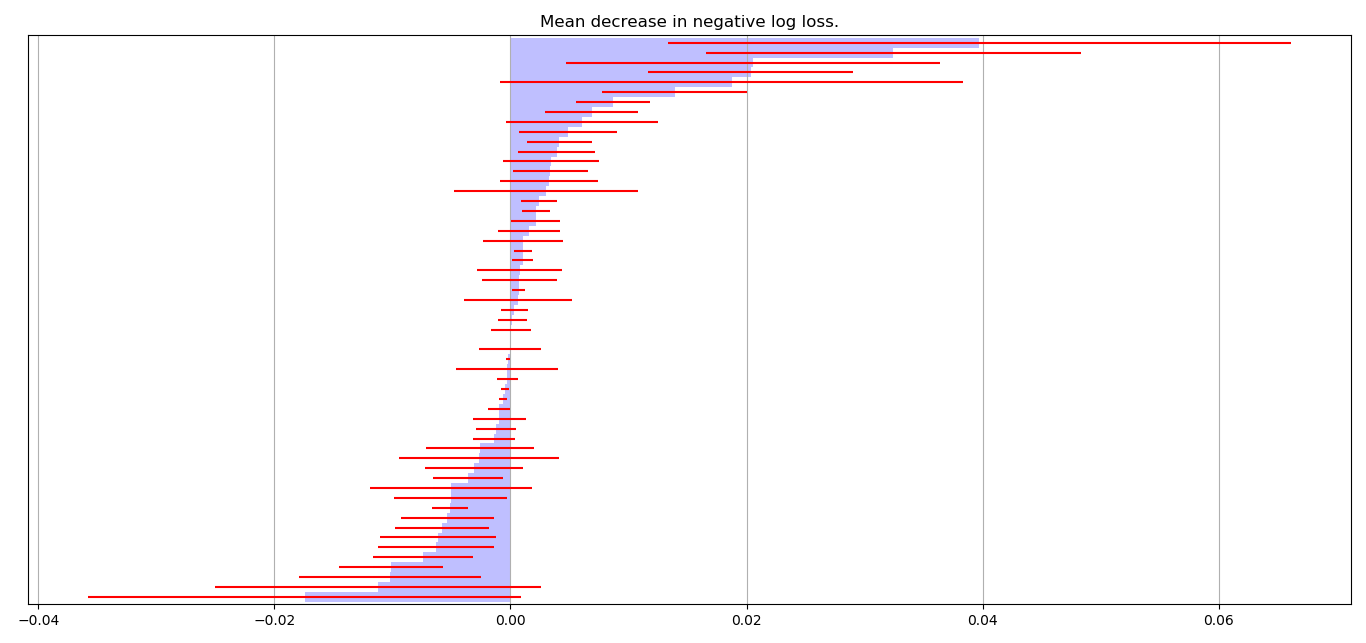
\includegraphics[width=1.35\textwidth, height=\textheight, keepaspectratio, angle=90]{results/images/feat_importance.png}
    \caption{Displays the mean feature importance loss in the bars. Each bar shows one feature. From the top to the bottom, there is one bar per feature in table \ref{table:feature_importance_results} and the rest are unimportant features. The standard deviation across cross validation folds is shown as a red line centered in the mean of each feature.}
    \label{fig:feat_importance}
\end{figure}

A new model was retrained using only these features. That model yields the results
in paragraph \emph{Performance metrics}. Also, as commented in
\ref{sec:methods_pipeline_feature_importance} it is important to explain how
these features are able to produce excess returns. It can be seen that price
related features are the ones that generate the higher mean of performance loss
and it means that a lot of market information is in prices already. Secondly, we
interpret that transacted volumes, both in currency and in bitcoins provide a lot
of information about market tendencies. As outlined in section \ref{sec:methods_features_sadf}
SADF related features determine when regime changes in price series occur and even
though that information is in prices, SADF offers a series that provides direct
information about changes towards explosive behavior. It is not surprising that
the day count until halving provides information and that is also connected with
the two volatility series. We have seen that close to halvings when
issuance changes and produces a considerable change in the network and that definitely
affects market volatility. Market capitalization offers an overall high level
market metric which provides an aggregated indicator of the market and similarly
does the transfer volume which accounts for the amount of currency that is flowing.
Making partitions over these features by means of a tree based model as bagging
ensembles are allows to generate complex relationship between them and identify
patterns. 

\paragraph{Performance metrics} Table \ref{table:perf_secondary_model}
shows the F1-score and negative log loss of the retrained secondary model.

\begin{table}[H]
  \centering
  \begin{tabular}{|c | c |} 
    \hline
    \multicolumn{2}{|c|}{Secondary model performance} \\
    \hline
    Metric & Value \\
    \hline
    F1-score                & 0.1574 \\
    \hline
    Negative log loss       & 0.6031 \\
    \hline
  \end{tabular}
  \caption{Secondary model classification metrics.}
  \label{table:perf_secondary_model}
\end{table}

F1-score evaluates model's accuracy when classifying samples. Negative log-loss
evaluates model's accuracy of the the estimated probabilities. The secondary
model will not be used as a classifier. Instead, predicted probabilities will
determine the bet size.